\documentclass{article}

\usepackage{array}
\usepackage{tikz}

\usetikzlibrary{shapes.multipart}
\usetikzlibrary{shapes.geometric}
\usetikzlibrary{arrows.meta}
\usetikzlibrary{positioning}
\usetikzlibrary{calc}

\usepackage[normalem]{ulem}

\tikzset{%
    pics/entity/.style n args={3}{code={%
        \node[draw,
        rectangle split,
        rectangle split parts=2,
        text height=1.5ex,
        ] (#1)
        {#2 \nodepart{second}
            \begin{tabular}{>{\raggedright\arraybackslash}p{8.5em}}
                #3
            \end{tabular}
        };%
    }},
    pics/weakentity/.style n args={3}{code={%
        \node[draw,
        rectangle split,
        rectangle split parts=2,
        text height=1.5ex,
        double,
        double distance = 0.07cm,
        rectangle split draw splits=false] (#1) {#2 \nodepart{two}
            \begin{tabular}{>{\raggedright\arraybackslash}p{8.5em}}
                #3
            \end{tabular}
        };%
        \draw[shorten <=0.05cm, shorten >=0.05cm] (#1.text split west) -- (#1.text split east);
    }},
    pics/relattribute/.style n args={2}{code={%
        \node[draw,
        text height=1.5ex,
        ] (#1)
        {#2};%
    }},
    pics/relationship/.style n args={2}{code={
        \node[draw,
        diamond,
        aspect=2,
        align=center,
        text height=1.5ex,
        ] (#1)
        {#2};%
    }},
    pics/defrelationship/.style n args={2}{code={
        \node[draw,
        diamond,
        aspect=2,
        align=center,
        text height=1.5ex,
        double,
        double distance = 0.07cm,
        ] (#1)
        {#2};%
    }},
    zig zag to/.style={% lines between entities and relationships
        to path={(\tikztostart) -| ($(\tikztostart)!#1!(\tikztotarget)$) |-
        (\tikztotarget)}
    },
    zig zag to/.default=0.5,
    one line/.style={% generic line
        zig zag to
    },
    one line arrow/.style={% generic line with an arrow at one end
        -{Classical TikZ Rightarrow[sharp, scale=2.5]},
        zig zag to
    },
    double line/.style={% for total participation (double lines)
        zig zag to, double, double distance = 0.07cm,
        shorten <=-0.07cm
    },
    double line arrow/.style={% for total participation, with an arrow
        -{Classical TikZ Rightarrow[sharp, scale=0.8]},
        zig zag to,
        double, double distance = 0.07cm,
        shorten <=-0.1cm, shorten >=0.04cm
    },
    dashed line/.style={% for relationship attributes
        zig zag to, dashed,
        shorten <=0.05cm
    },
    specialization/.style={% for specialization
        -{Latex[round,open,scale=2]}, zig zag to
    }
}\begin{document}
    \begin{center}
        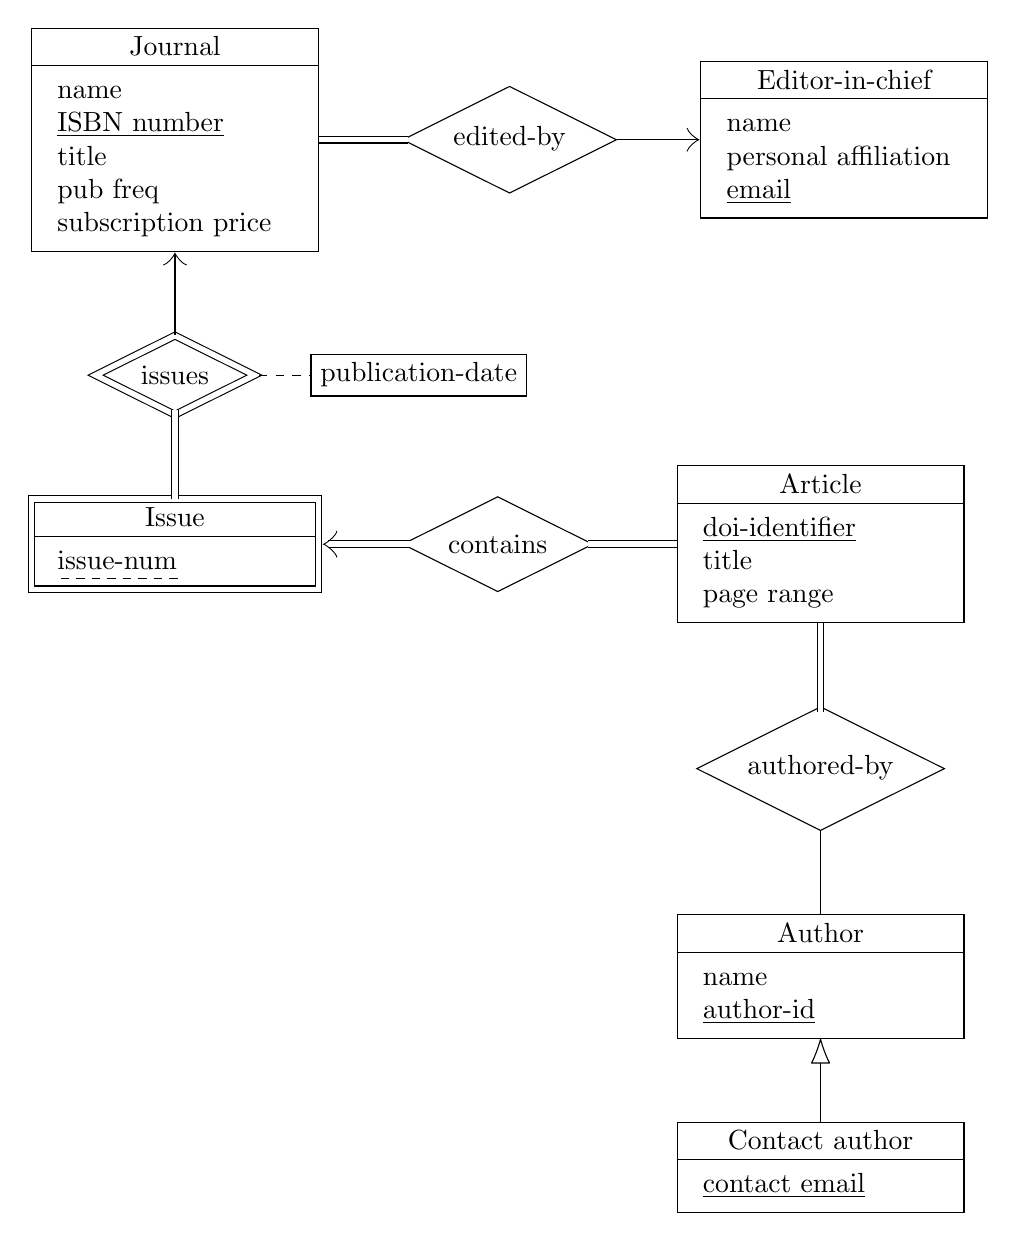
\begin{tikzpicture}
            \pic {entity={140328131125200}{Journal}{%
                name\\
                \underline{ISBN number}\\
                title\\
                pub freq\\
                subscription price\\
            }};
            \pic[right=3em of 140328131125200] {relationship={140328132235072}{edited-by}};
            \pic[right=3em of 140328132235072] {entity={140328131125104}{Editor-in-chief}{%
                name\\
                personal affiliation\\
                \underline{email}\\
            }};
            \draw[double line] (140328132235072.west) -- (140328131125200.east);
            \draw[one line arrow] (140328132235072.east) -- (140328131125104.west);
            \pic[below=3em of 140328131125200] {defrelationship={140328132235072}{issues}};
            \pic[below=3em of 140328132235072] {weakentity={140328131125056}{Issue}{%
                \dashuline{issue-num}\\
            }};
            \draw[one line arrow] (140328132235072.north) -- (140328131125200.south);
            \draw[double line] (140328132235072.south) -- (140328131125056.north);
            \pic[right=2em of 140328132235072] {relattribute={a140328132235072}{%
                publication-date
            }};
            \draw[dashed line] (140328132235072.east) -- (a140328132235072.west);
            \pic[right=3em of 140328131125056] {relationship={140328132235072}{contains}};
            \pic[right=3em of 140328132235072] {entity={140328131123856}{Article}{%
                \underline{doi-identifier}\\
                title\\
                page range\\
            }};
            \draw[double line arrow] (140328132235072.west) -- (140328131125056.east);
            \draw[double line] (140328132235072.east) -- (140328131123856.west);
            \pic[below=3em of 140328131123856] {relationship={140328132235072}{authored-by}};
            \pic[below=3em of 140328132235072] {entity={140328132233776}{Author}{%
                name\\
                \underline{author-id}\\
            }};
            \draw[double line] (140328132235072.north) -- (140328131123856.south);
            \draw[one line] (140328132235072.south) -- (140328132233776.north);
            \pic[below=3em of 140328132233776] {entity={140328132232288}{Contact author}{%
                \underline{contact email}\\
            }};
            \draw[specialization] (140328132232288.north) -- (140328132233776.south);
        \end{tikzpicture}
    \end{center}
\end{document}
